% Summary of aksenova2024: The computational power of harmonic forms

\begin{abstract}
\begin{enumerate}
  \item Argues that while completely overlapping, embedded, and disjoint phonological tiers are attested, partially overlapping tiers are not.
  \item Surveys subregular classes for phonological \textit{processes} (Input-TSL, Output-TSL), and the phonotactic patterns they capture.
\end{enumerate}
\end{abstract}

\section*{Subregular processes}

\subsection*{Input Strictly-Local}

For any input symbol \textit{x}, its output string \textit{u} will depend only on \textit{x} and the previous \textit{k-1} elements in the input string.

\begin{center}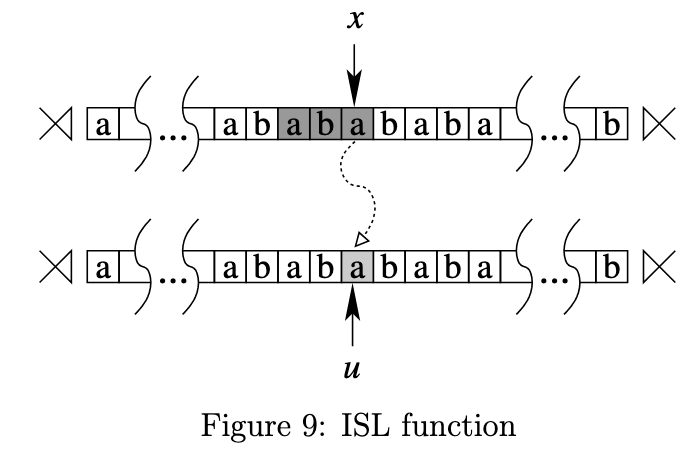
\includegraphics[width=0.80\linewidth]{images/pasted-20260915064949.png}\end{center}

\subsection*{Output Strictly-Local}

In LOSL and ROSL functions, the context is a bounded chunk of the output instead:

\begin{center}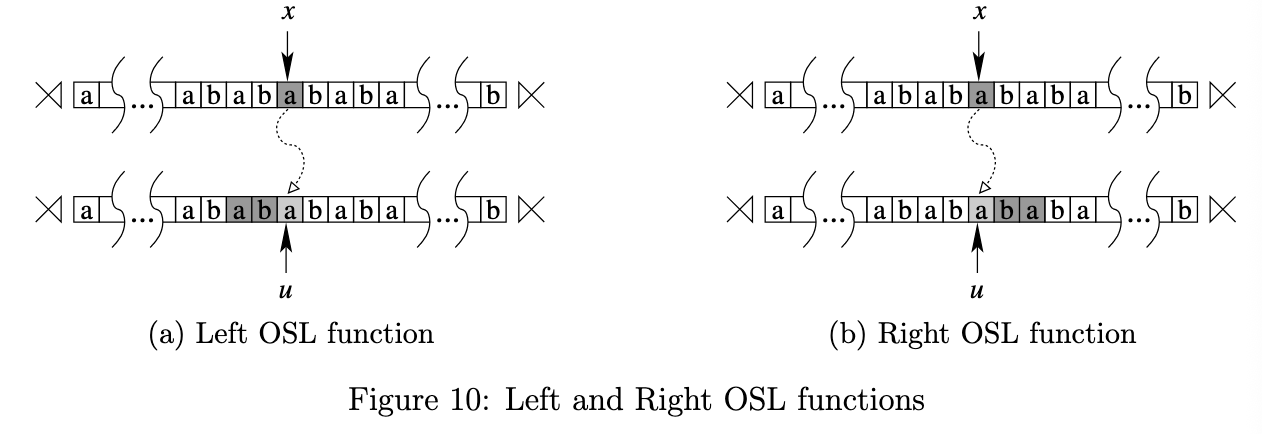
\includegraphics[width=0.80\linewidth]{images/pasted-20260915065017.png}\end{center}

Progressive and Regressive patterns go here (Chandlee 2014).

\section*{Phonotactic patterns}

Output Strictly-Local:

\begin{itemize}
  \item Progressive Harmony (first vowel determines all others)
  \item Regressive Harmony (last vowel determines all others)
\end{itemize}

Weakly Deterministic:

\begin{itemize}
  \item Dominant-Recessive Harmony (everything harmonizes if a specific value is present anywhere)
\end{itemize}

Subregular but not Weakly Deterministic:

\begin{itemize}
  \item Sour Grapes Patterns (non-intervening blockers; unattested)
  \item Circumambient Unbounded (surrounding triggers)
\end{itemize}

Majority Rules also unattested.
